\chapter{Experiment}
\todo{ne tolle Einleitung schreiben}

\section{Setup A: Estimation of the quadrature point of the MZI modulator}
To calculate the quadrature point of the used MZI modulator the setup shown in figure \ref{fig:A_setup}\footnote[3]{Luca Alloatti, Materials for the preparation of OKT lab 8} was used. A laser source with an output wavelength of 1550~nm and an output power of 0~dBm was connected to an MZI modulator. The output of the MZI modulator was connected to a power meter. The modulator was biased over a variable DC voltage.

The DC voltage was swept from -4.8~V to 5.1~V in steps of 0.3~V. At every point the output power of the MZM was measured.

\begin{figure}%
\centering
\includegraphics[width=.6\columnwidth]{Grafiken/SetupA.png}%
\caption{Setup A}%
\label{fig:A_setup}%
\end{figure}

\begin{figure}%
\centering
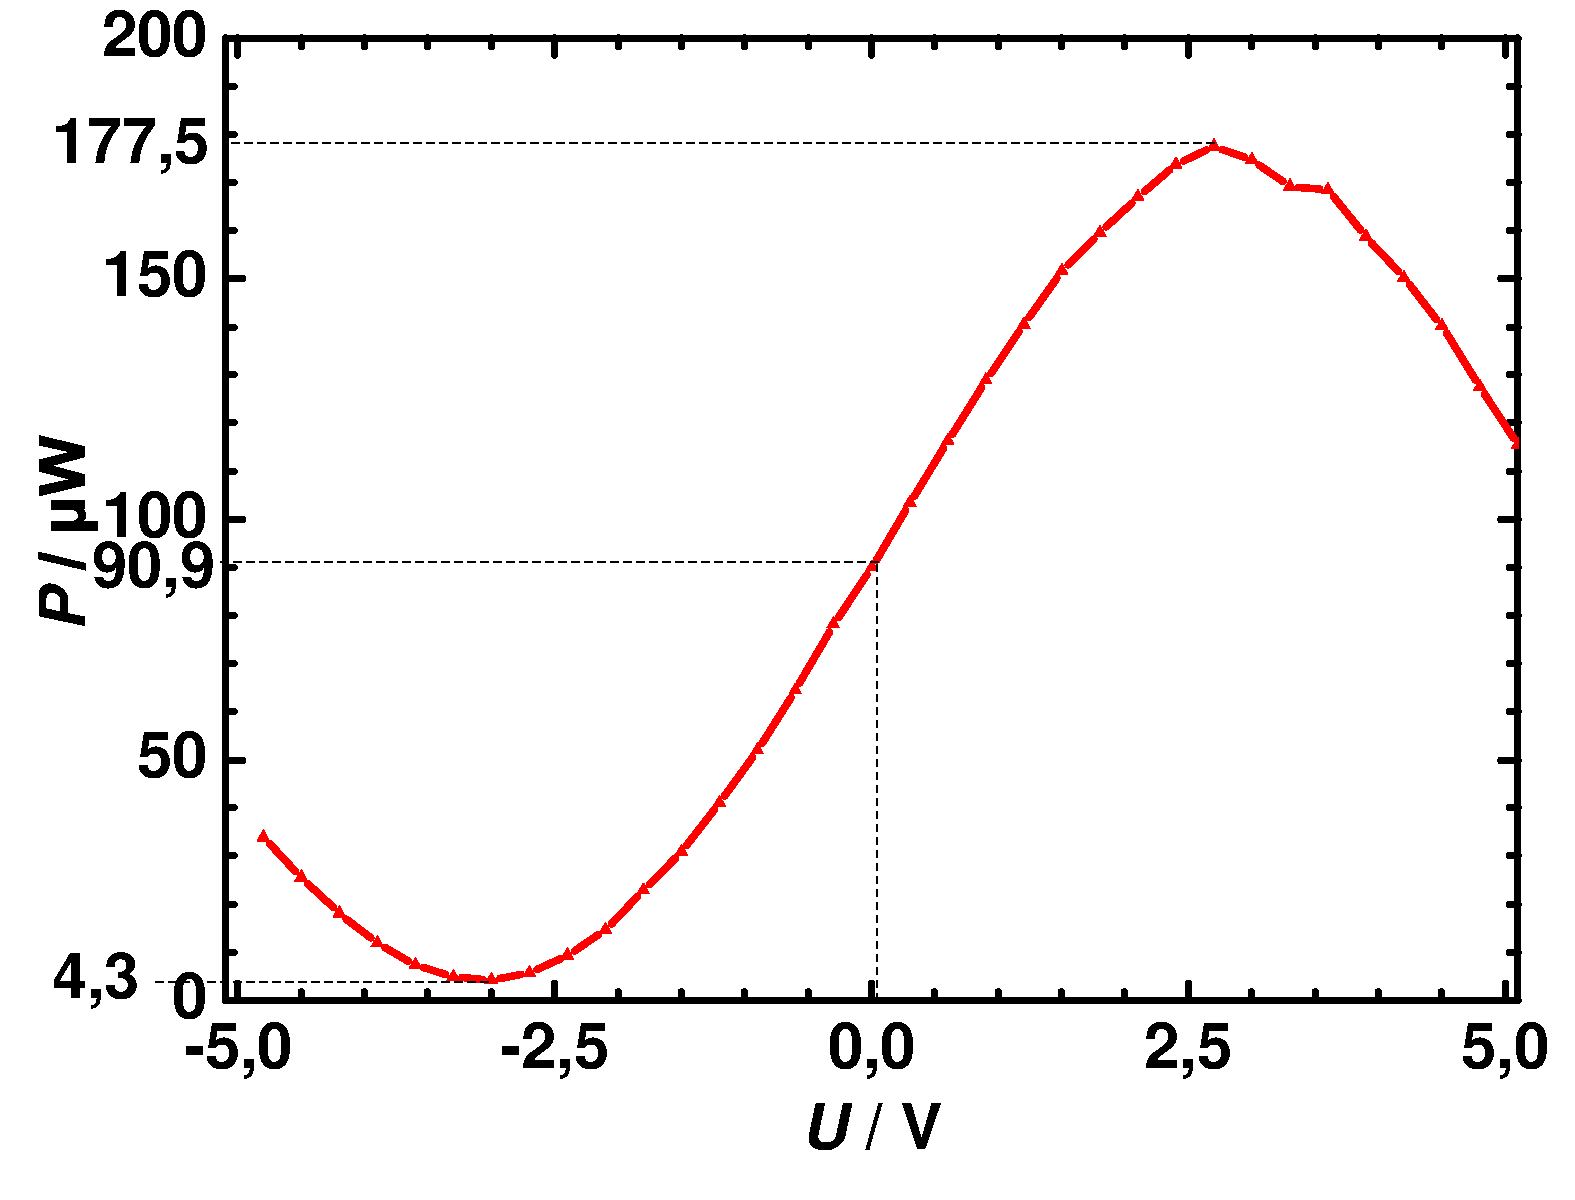
\includegraphics[width=.6\columnwidth]{Grafiken/A_quadratur.pdf}%
\caption{}%
\label{fig:A_quadratur}%
\end{figure}

 Figure \ref{fig:A_quadratur} shows the recorded $P$/$U$ curve. It shows a good accordance to the squared sine $P$/$U$ curve of a theoretical MZI modulator.
The maximum optical output power of the MZI is at 